\documentclass[a4paper]{article}

% LaTeX preambule: loading relevant packages, configuring Python listings
\usepackage{graphicx}
\usepackage{amsmath}
\usepackage{color}
\usepackage{listings}
\usepackage{hyperref}
\usepackage{graphicx}
\usepackage{epstopdf}
\usepackage{inputenc}
\usepackage{bm}
\usepackage{subcaption}
\usepackage{tabto}
\def\signed#1{{\unskip\nobreak\hfil\penalty50
    \hskip2em\hbox{}\nobreak\hfil\sl#1
    \parfillskip=0pt \finalhyphendemerits=0 \par}}
\usepackage[a4paper, total={6in, 8in}]{geometry}

\title{%
  Understanding Optical Diffraction and Interference Patterns through a Historical Perspective}
\author{PH2255 Final Report\\ \\Candidate 2104412}

\definecolor{dkgreen}{rgb}{0,0.6,0}
\definecolor{gray}{rgb}{0.5,0.5,0.5}
\definecolor{mauve}{rgb}{0.58,0,0.82}

% Settings for colour-coding and formatting Python code:
\lstset{
  language=Python,                % the language of the code
  basicstyle=\footnotesize,           % the size of the fonts that are used for the code
  numbers=left,                   % where to put the line-numbers
  numberstyle=\tiny\color{gray},  % the style that is used for the line-numbers
  stepnumber=5,                   % the step between two line-numbers. If it's 1, each line
                                  % will be numbered
  numbersep=5pt,                  % how far the line-numbers are from the code
  backgroundcolor=\color{white},      % choose the background color. You must add \usepackage{color}
  showspaces=false,               % show spaces adding particular underscores
  showstringspaces=false,         % underline spaces within strings
  showtabs=false,                 % show tabs within strings adding particular underscores
  frame=single,                   % adds a frame around the code
  rulecolor=\color{black},        % if not set, the frame-color may be changed on line-breaks within not-black text (e.g. commens (green here))
  tabsize=2,                      % sets default tabsize to 2 spaces
  captionpos=b,                   % sets the caption-position to bottom
  breaklines=true,                % sets automatic line breaking
  breakatwhitespace=false,        % sets if automatic breaks should only happen at whitespace
  title=\lstname,                   % show the filename of files included with \lstinputlisting;
                                  % also try caption instead of title
  keywordstyle=\color{blue},          % keyword style
  commentstyle=\color{dkgreen},       % comment style
  stringstyle=\color{mauve},         % string literal style
  escapeinside={\%*}{*)},            % if you want to add LaTeX within your code
  morekeywords={*,...}               % if you want to add more keywords to the set
}

\begin{document}
\maketitle

\begin{abstract}
Abstract
\end{abstract}

\tableofcontents
\newpage
\section{Introduction}
To fully understand an optical theory of light---and to understand why diffraction and interference experiments are so important to ir---it is helpful to understand the history of how different theories arose. Today, we have a very good understanding of light as an electromagnetic interaction between the magnetic and electric fields, enabled by Photons---the EM force carrier. It is common knowledge, even in popular culture, that light exhibits both wave-like and particle-like behaviour. However, in the 17\textsuperscript{th} and 18\textsuperscript{th}, the picture wasn't so clear.

\subsection{A Brief Historical Overview}

While ancient philosiphers---such as Pythagoras, Plato, and Asristotle---began the development of theories of light in the Greek Classical period, progress rapidly accelerated in the seventeenth century with the advent of the refracting telescope. As Galileo and Kepler developed their respective telescope systems in the early 1600s, Snel\footnote{Willebrord Snellius, usually known as Snell} re-discovered Sahl's law of refraction. While these laws did accurately describe light moving through media of varying refractive indices, they rely on the assumption that light travels the path which takes the least time. This assumption can be disproven, such as with a spherical mirror, and as such cannot define a fundemental theory of light

Nonetheless, Snel's law laid the foundations for a rapid development of modern optics. In 1665, at the Royal Society in London, Hooke was one of the first to study the field known today as diffraction and interference, the subject of this report. In his book \emph{Micrographia} \cite{gut:hooke}, the idea of light being vibrations in a medium was first proposed:
\begin{quote}
  \it{
  ``\ldots this motion is propagated every way with equal velocity, whence necessarily every pulse or vibration of the luminous body will generate a Sphere, which will continually increase, and grow bigger, just after the same manner (though indefinitely swifter) as the waves or rings on the surface of the water do swell into bigger and bigger circles about a point of it, where by the sinking of a Stone the motion was begun, whence it necessarily follows, that all the parts of these Spheres undulated through a Homogeneous medium cut the Rays at right angles.''}
  \signed{\emph{---\cite{gut:hooke}}}
\end{quote}
Thus began the wave theory of light. 
\subsection{Newton's Particle Theory}

At the same time, Newton was making his own advances in the field of optics. In his 1704 paper \emph{Opticks} \cite{gut:newt}, he proposed a particle theory of light---initially set forward by Descartes---where light rays are comprised of small discrete particles named ``corpuscules'', hence its name \emph{the corpuscular theory}. His main motivation for choosing a particle theory was the apparent inability of a wave theory to explain rectilinear propagation\footnote{The propensity of light to travel in a straight line in the absence of any interference.}.

Despite the corpuscular theory's ability to describe both rectilinear propagation and polarisation (whereas wave theories ignored the latter), it relied on assumptions that modern physicists would resoundly reject - that the speed of light is infinite, but also that it sped up in denser media. 
\subsection{Huygens' Wave Theory}



\subsection{Developing an Optical Theory}

\section{Experimental Setup}

\section{Experimental Method}

\section{Results}

\section{Data Analysis}

\section{Summary of Findings}

Text \lstinline$inline$
\begin{lstlisting}
# Codeblock
\end{lstlisting}
\begin{equation}
\text{equation}
\end{equation}

\begin{figure}[h]
%\centerline{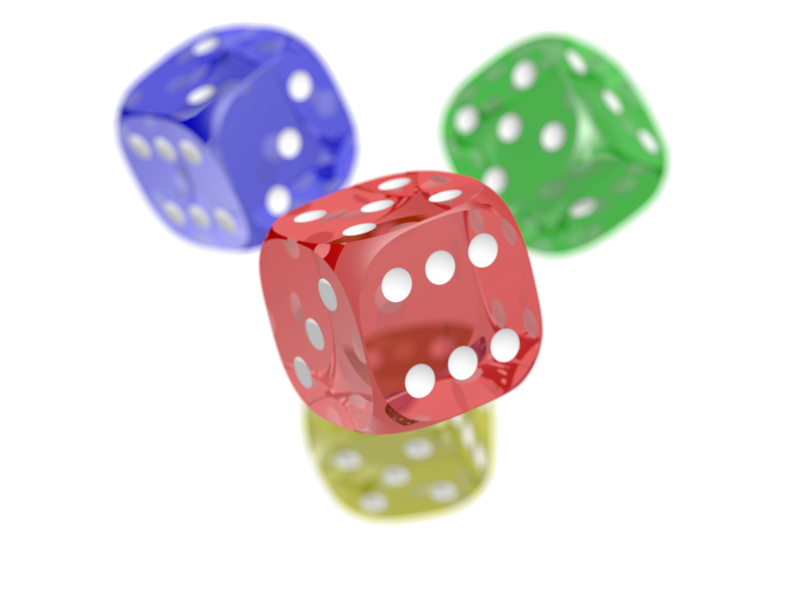
\includegraphics[scale=0.3]{png.png}}
\caption{PNG}
\label{fig:png}
\end{figure}

\begin{table}[h!]
\centering
\begin{tabular}{lll}
\hline
Table & Table & Table\\ \hline
Table & Table & Table \\
Table & Table & Table \\
\end{tabular}
\caption{\label{tab:table}Caption.}
\end{table}
\newpage
\begin{appendix}
\section{Appendix}
\subsection{Bibliography}
\bibliographystyle{plainnat}
\bibliography{export}
\subsection{Python Code}\label{sec:python}
%\lstinputlisting[language=Python,frame=single]{py.py}%

\end{appendix}

\end{document}
